\documentclass{beamer}
\usefonttheme[onlymath]{serif}

\usepackage{amsfonts}

% Code Block Setting
\usepackage{listings}
\lstset{language=C,
numberstyle=\footnotesize,
basicstyle=\ttfamily\footnotesize,
numbers=left,
stepnumber=1,
frame=shadowbox,
breaklines=true}

\usetheme{Warsaw}
% \usecolortheme{dove}

% Add frame number and total frame number in footline
\defbeamertemplate*{footline}{shadow theme}{%
    \leavevmode%
    \hbox{\begin{beamercolorbox}[wd=.5\paperwidth,ht=2.5ex,dp=1.125ex,leftskip=.3cm plus1fil,rightskip=.3cm]{author in head/foot}%
            \usebeamerfont{author in head/foot}\hfill\insertshortauthor
        \end{beamercolorbox}%
        \begin{beamercolorbox}[wd=.4\paperwidth,ht=2.5ex,dp=1.125ex,leftskip=.3cm,rightskip=.3cm plus1fil]{title in head/foot}%
            \usebeamerfont{title in head/foot}\insertshorttitle\hfill%
        \end{beamercolorbox}%
        \begin{beamercolorbox}[wd=.1\paperwidth,ht=2.5ex,dp=1.125ex,leftskip=.3cm,rightskip=.3cm plus1fil]{title in head/foot}%
            \hfill\insertframenumber\,/\,\inserttotalframenumber
    \end{beamercolorbox}}%
    \vskip0pt%
}

% Tikz related
\usepackage{tikz}
\usetikzlibrary{fit}
\usetikzlibrary{calc}
\usetikzlibrary{positioning}

% Number the figures
\setbeamertemplate{caption}[numbered]

% Add outline page at begining of each section
\AtBeginSection[]
{
    \begin{frame}<beamer>
        \frametitle{Outline}
        \tableofcontents[currentsection, hideallsubsections]
    \end{frame}
}

%%%%%%%%%%%%%%%%%%%%%%%%%%%%%%%%%%%%%%%%%%%%%

\title{High-performance Energy-efficient Recursive Dynamic Programming with Matrix-multiplication-like Flexible Kernels}
\author{
    Jesmin Jahan Tithi\inst{1},\\
    Pramod Ganapathi \inst{1},\\
    Sonal Aggarwal\inst{1},\\
    Rezaul Chowdhury\inst{1}
}
\institute{
    \inst{1} Department of Computer Science, Stony Brook University, New York, 11790-4400, USA
}
\date{
    \tiny{2015 IEEE 29th International Parallel and Distributed Processing Symposium}\\
    \tiny{Presented by ShiangYun Yang}
}

\begin{document}
\begin{frame}
    \titlepage
\end{frame}

\section{Introduction}

\subsection{SIMD}
\begin{frame}
    \frametitle{SIMD}
	\begin{itemize}
		\item Single instruction multiple data
		\item without threads support
	\end{itemize}
\end{frame}


\subsection{VPU}
\begin{frame}
    \frametitle{VPU}
	\begin{itemize}
		\item Vector processing units 
		\item combine itstructions as vector	
	    \begin{figure}
			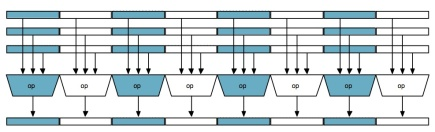
\includegraphics[scale=0.5]{figure/vpu.jpg}
		\end{figure}
	\end{itemize}
\end{frame}


\section{Algorithm}

\subsection{Constraint Condition}
\begin{frame}
    \frametitle{Constraint Condition}
    \begin{itemize}
		\item Assume $n = 2^t$ for some integer $t \ge 0$ for all problems.
		\item The size of DP table is $n \times n$.
	\end{itemize}
\end{frame}

\subsection{Parenthesization Problem}
\begin{frame}
    \frametitle{Parenthesization Problem}
    \begin{figure}
		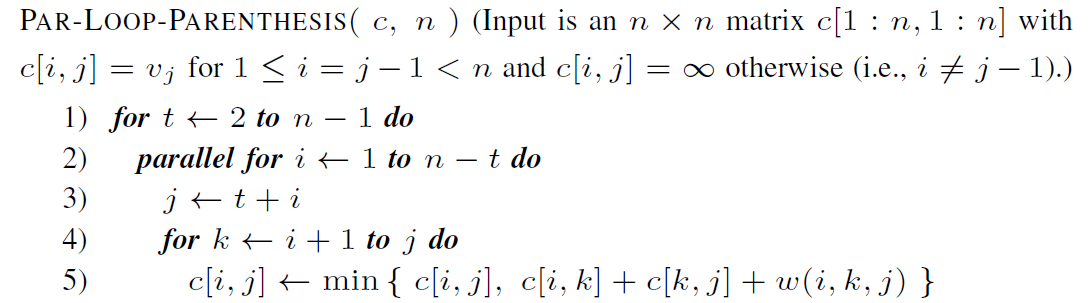
\includegraphics[scale=0.4]{figure/fig-parenthesis.png}
	\end{figure}
    \begin{itemize}
    	\item $w(i, k, j)$ returns the cost of combining parenthesizations of
    		$x_i \; \cdots x_k$ and $x_k \; \cdots x_j$
    	\item The optimal parenthesizing cost $c[1, n]$ for the entire sequence.
    \end{itemize}
\end{frame}

\subsection{Parenthesization Problem - Parallel CORDAC}
\begin{frame}
    \frametitle{Parallel CORDAC Algorithm - Func A, B}
    \begin{figure}
		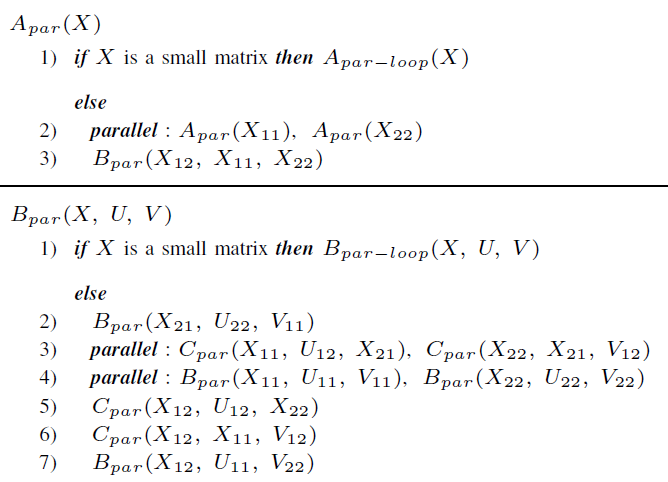
\includegraphics[scale=0.5]{figure/fig-parenthesis-parallel-1.png}
	\end{figure}
\end{frame}

\begin{frame}
    \frametitle{Parallel CORDAC Algorithm - Func C}
    \begin{figure}
		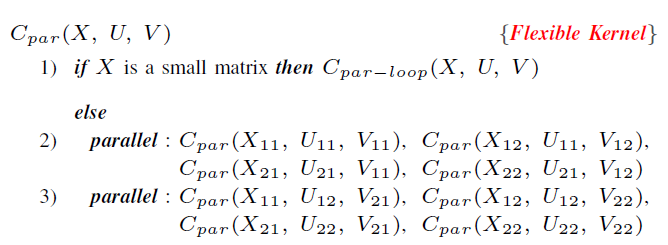
\includegraphics[scale=0.5]{figure/fig-parenthesis-parallel-2.png}
	\end{figure}
\end{frame}

\begin{frame}
    \frametitle{Parallel CORDAC Algorithm Figure}
    \begin{figure}
        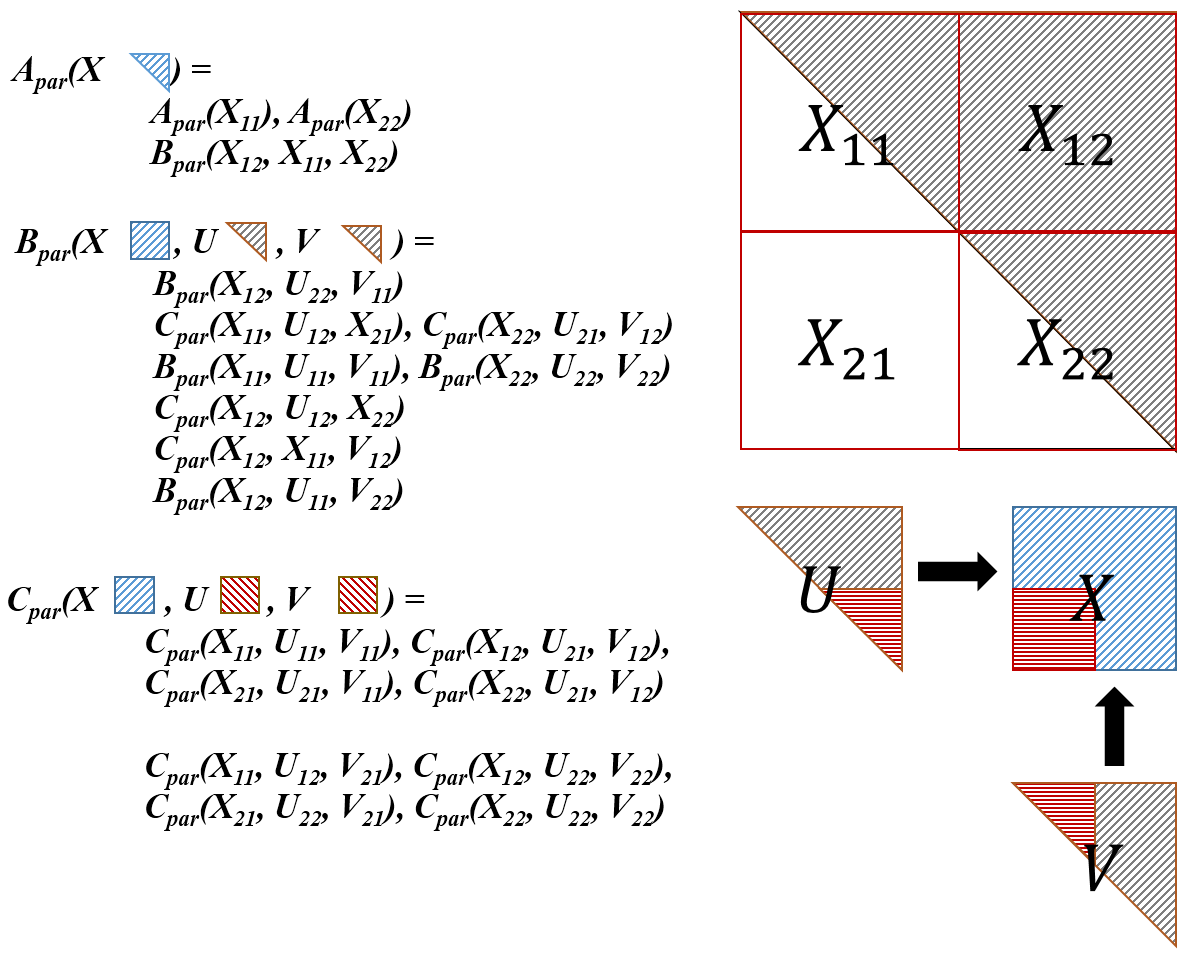
\includegraphics[scale=0.25]{figure/fig-par-explain.png}
    \end{figure}
\end{frame}

\subsection{Other Problems}
\begin{frame}
    \frametitle{Other Problems}
    \begin{figure}
		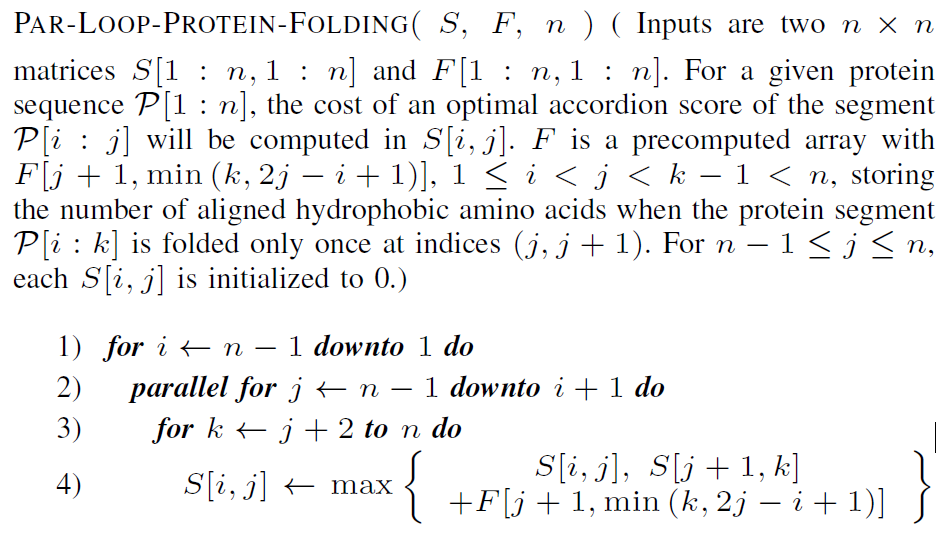
\includegraphics[scale=0.2]{figure/fig-folding.png}
	\end{figure}
	\begin{figure}
		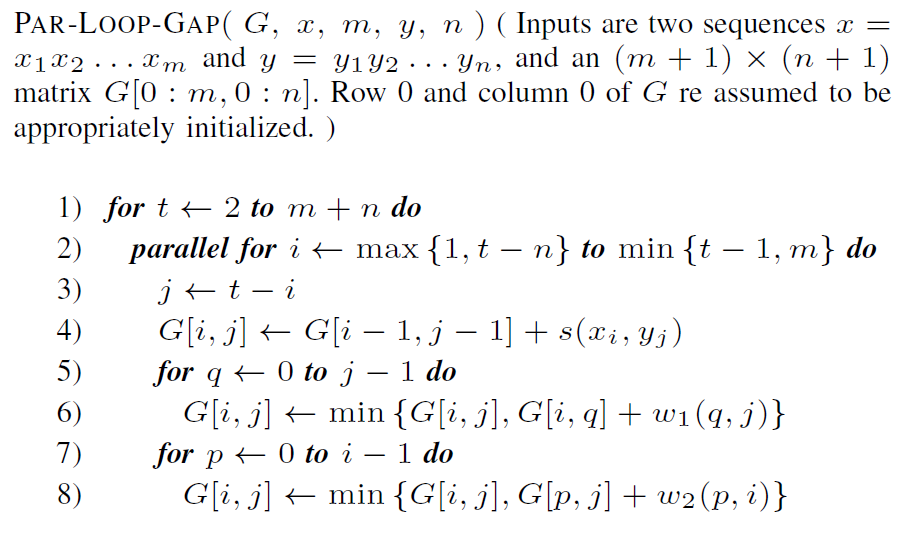
\includegraphics[scale=0.2]{figure/fig-gap.png}
	\end{figure}
\end{frame}

\subsection{Other Problems - Parallel CORDAC}
\begin{frame}
    \frametitle{Other Problems - Parallel CORDAC}
    \begin{figure}
		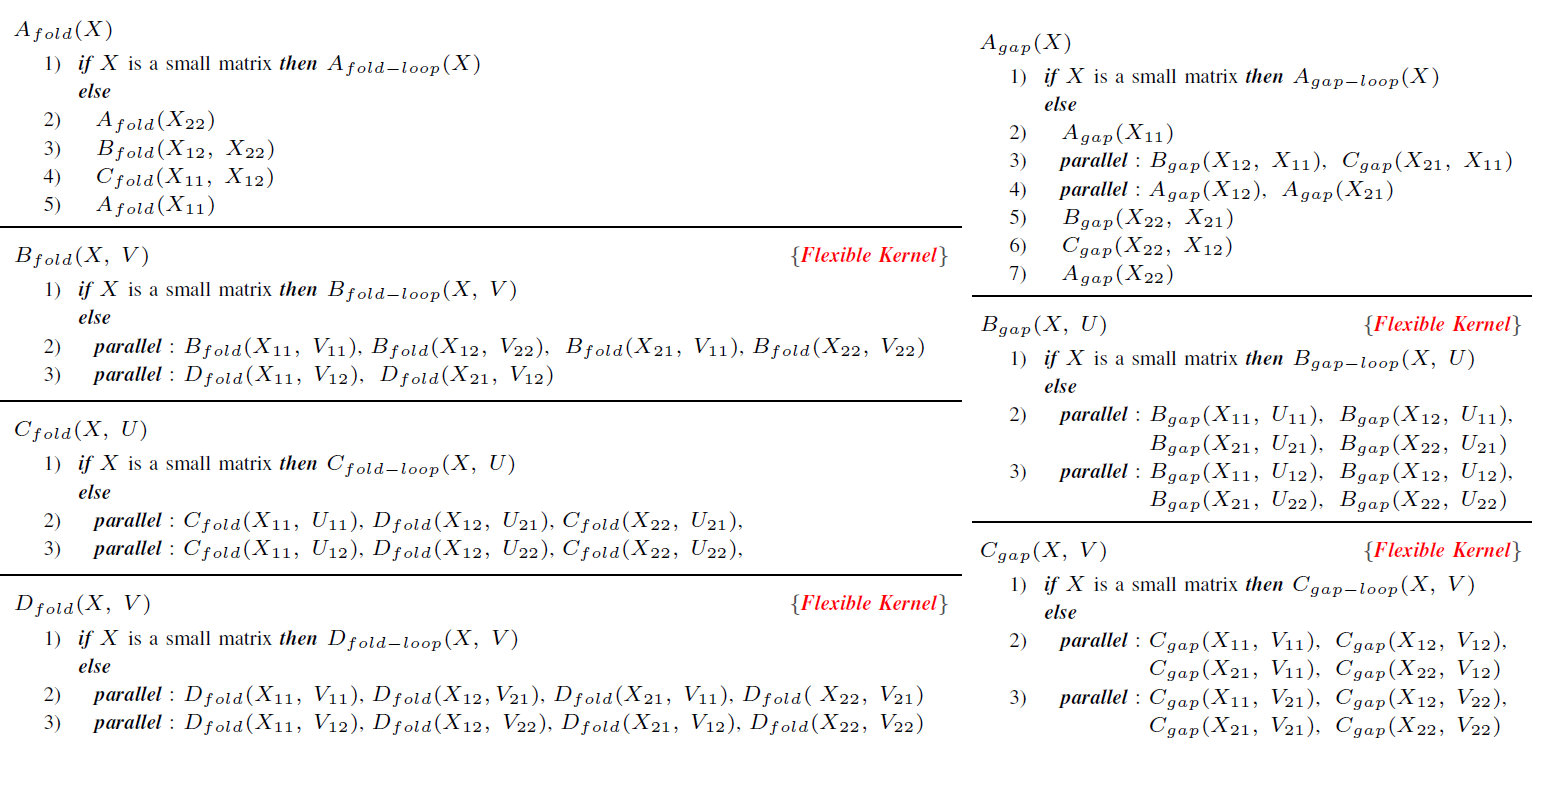
\includegraphics[scale=0.2]{figure/fig-fold-gap-parallel.png}
	\end{figure}
\end{frame}

\begin{frame}
    \frametitle{Other Problems - Parallel CORDAC}
    \begin{figure}
		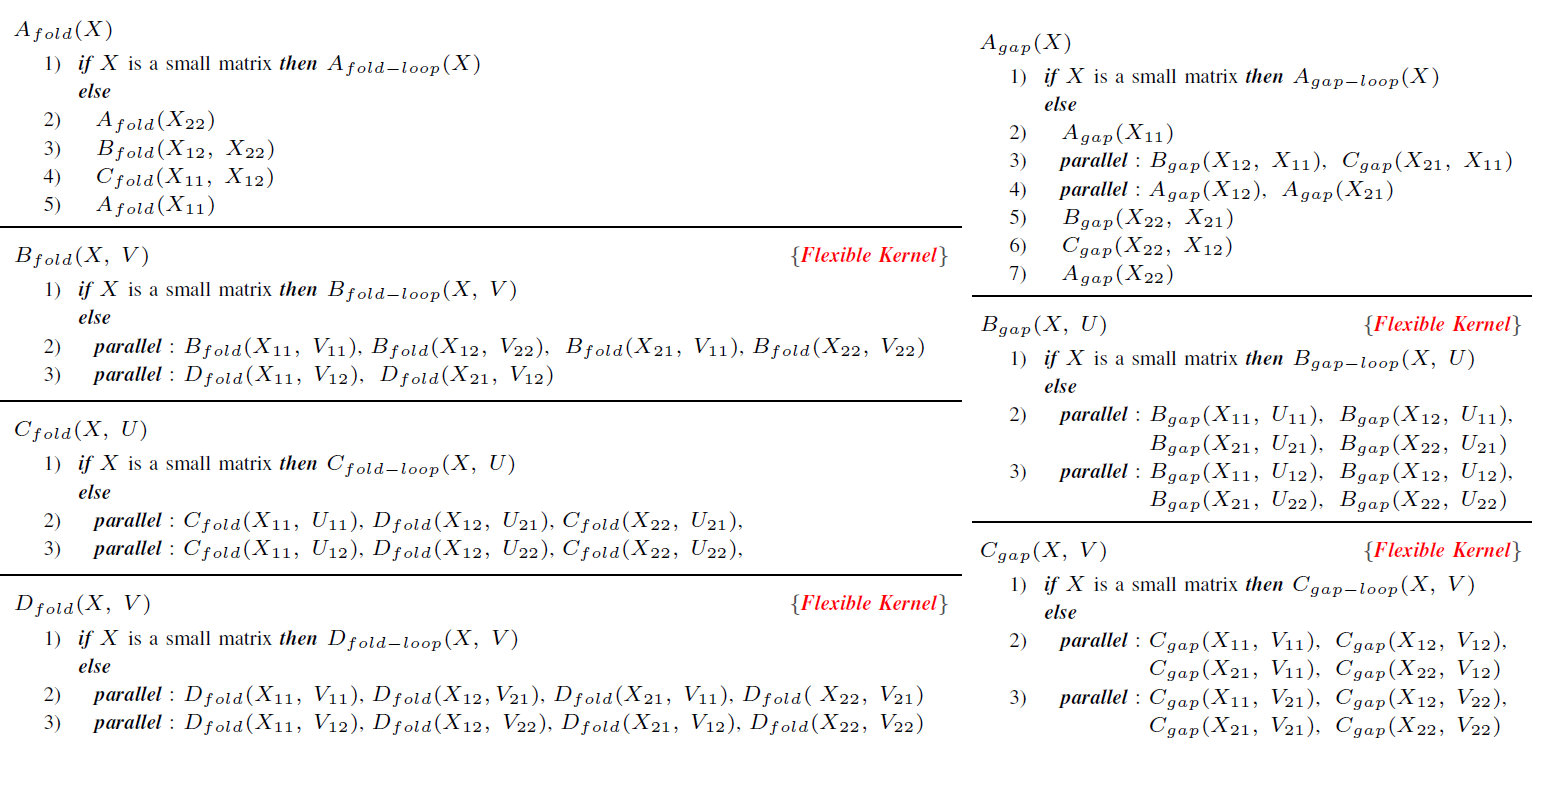
\includegraphics[scale=0.2]{figure/fig-fold-gap-parallel.png}
	\end{figure}
\end{frame}

\section{Complexity Analysis}

\subsection{Complexity Analysis}
\begin{frame}
    \frametitle{Serial Cache Complexity Analysis}
    \begin{itemize}
    	\item $Q_f(n)$ denote the cache complexity of $f_{par}$ on a matrix of size $n \times n$
    	\item $f \in \left\{ A, B, C \right\}$
    \end{itemize}
    \begin{align*}
		Q_f(n) &= \mathcal{O}(n + n^2 / B) 
			&& \text{if } n^2 \le \gamma_f M, \; \gamma_f \in (0, 1 ] \\
		Q_A(n) &= Q_A(n/2) + Q_B(n/2) \\
		Q_B(n) &= 4 Q_B(n/2) \\
		Q_C(n) &= 8 Q_C(n/2)
    \end{align*}
    \begin{align*}
    	&\Rightarrow Q_A(n) = \mathcal{O}\left(n + n^2/B + n^3 /M + n^3 / \left(B \sqrt{M}\right)  \right)
  	\end{align*}
\end{frame}

\begin{frame}
    \frametitle{Span Analysis}
    \begin{itemize}
    	\item $T_f(n)$ denote the span complexity of $f_{par}$ on a matrix of size $n \times n$
    	\item $f \in \left\{ A, B, C \right\}$
    \end{itemize}
    \begin{align*}
		T_f(n) &= \Theta(1)
			&& \text{if } n = 1 \\
		T_A(n) &= T_A(n/2) + T_B(n/2) + \Theta(1) \\
		T_B(n) &= 3 (T_B(n/2) + T_C(n/2)) + \Theta(1) \\
		T_C(n) &= 2 T_C(n/2) + \Theta(1)
    \end{align*}
    \begin{align*}
    	& \Rightarrow T_A(n) = \mathcal{O}\left(n^{\log_2 3}\right)
  	\end{align*}
\end{frame}

\subsection{Complexity Table}
\begin{frame}
    \frametitle{Complexity Table}
    \begin{figure}
		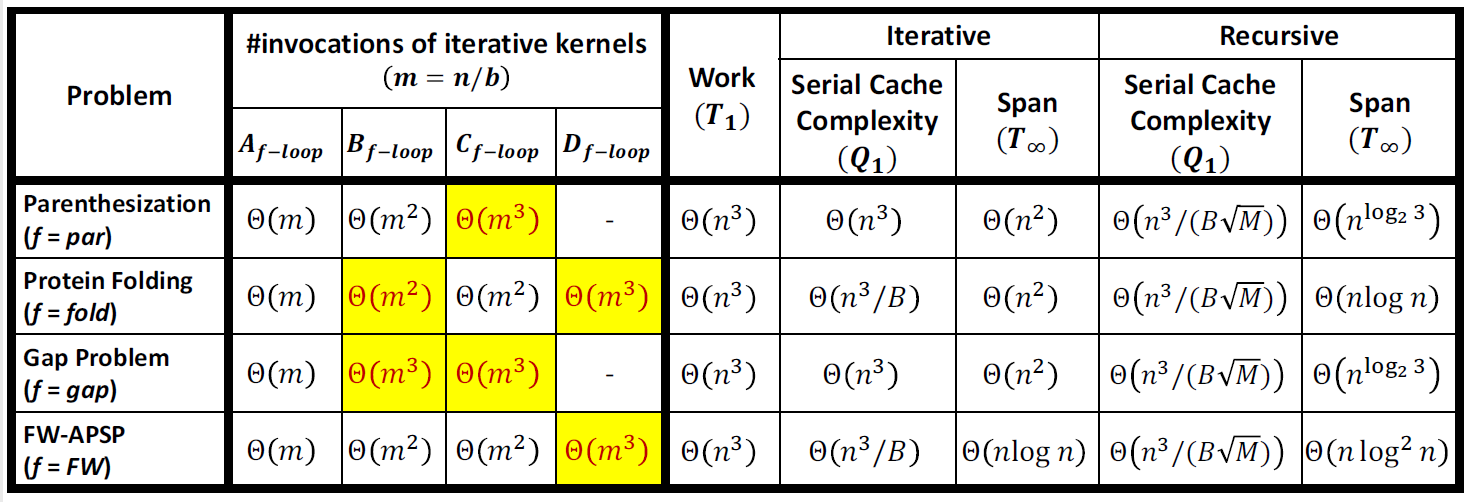
\includegraphics[scale=0.25]{figure/fig-complexity.png}
	\end{figure}
    \begin{itemize}
		\item size of cache $M$, cache line size $B$, processing elements $p$
		\item Runtime $T_p = \mathcal{O}(T_1/p + T_{\infty})$
		\item Cache complexity $Q_p = \mathcal{O}(Q_1 + p(M/B) T_{\infty})$
	\end{itemize}
\end{frame}
\section{Optimization}

\subsection{Hybrid CORDAC}
\begin{frame}
    \frametitle{Hybrid CORDAC}
		Cache-efficient algorithm recursive subdivision continues until 
		the problem size becomes small enough.
	\begin{itemize}
		\item Benefits of both iterative and recursive algorithms
		\item Asymptotic improvement in parallelism
		\item Highly optimizable base cases
	\end{itemize}
\end{frame}

\subsection{Optimizing Kernel Functions}
\begin{frame}
    \frametitle{Optimizing Kernel Functions}
	\begin{description}
		\item[Copy-optimization] Copy the data into local $b \times b$ 
			static arrays inside the kernel.
		\item[Loop Reordering] In flexible kernels, it is possible to change
			the looping order without hampering the correctness of the algorithm.
	\end{description}
\end{frame}

\subsection{Data Layout}
\begin{frame}
    \frametitle{Data Layout}
	\begin{figure}
		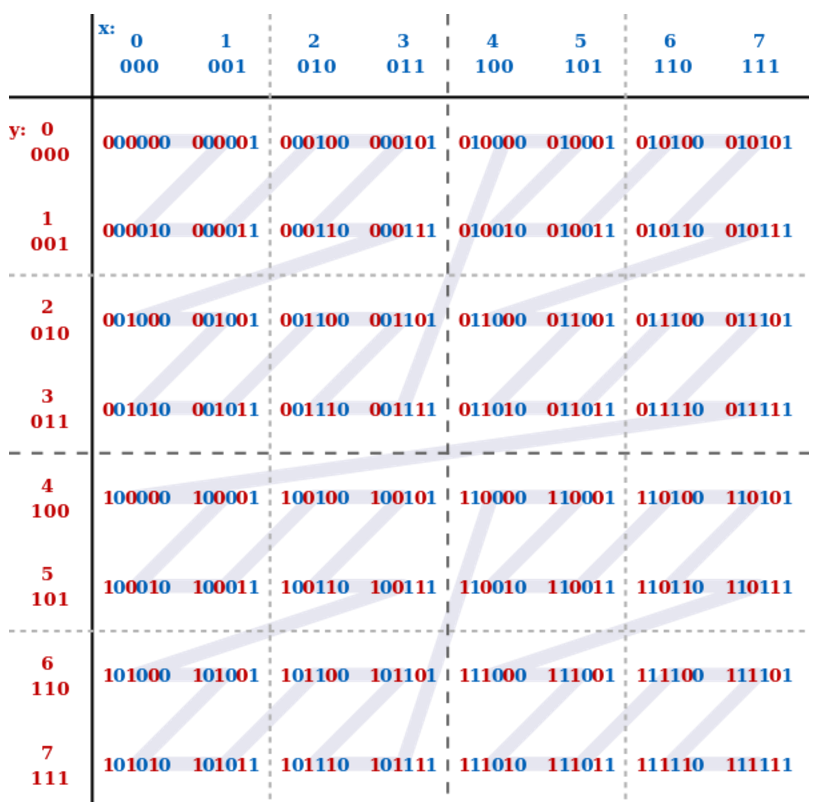
\includegraphics[scale=0.2]{figure/fig-z-morton.png}
	\end{figure}
	\begin{itemize}
		\item \textit{Z-Morton Row-Major}(ZM\_RM) layout is beneficial because
			it improves both temporal and spatial localities.
	\end{itemize}
\end{frame}

\subsection{Auto vs. Explicit Vectorization}
\begin{frame}
    \frametitle{Auto vs. Explicit Vectorization}
    It often vectorize the base-case of the dominating kernel.
	\begin{itemize}
		\item For example, $C_{\textit{loop}}$ is enough to get the 
			major share of the speedup.
	\end{itemize}
\end{frame}
\section{Experiment}

\subsection{Sparse Matrices}
\begin{frame}
	\frametitle{Sparse Matrices}
	\begin{figure}
		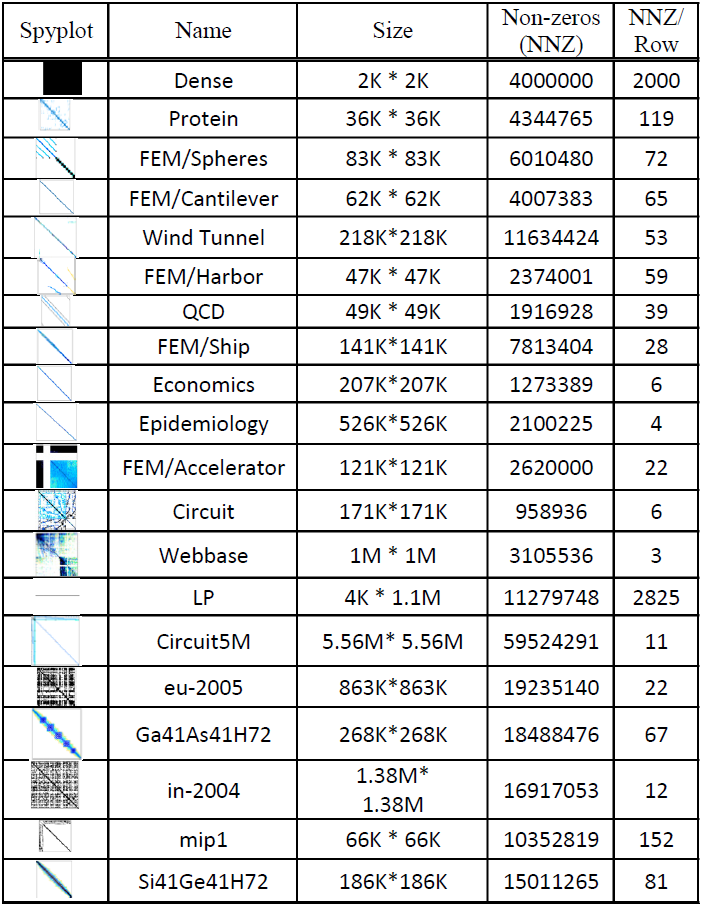
\includegraphics[scale=0.25]{figure/fig5-kindmatrices.png}
	\end{figure}
\end{frame}

\subsection{Memory Footprint}
\begin{frame}
	\frametitle{Memory Footprint}
	\begin{figure}
		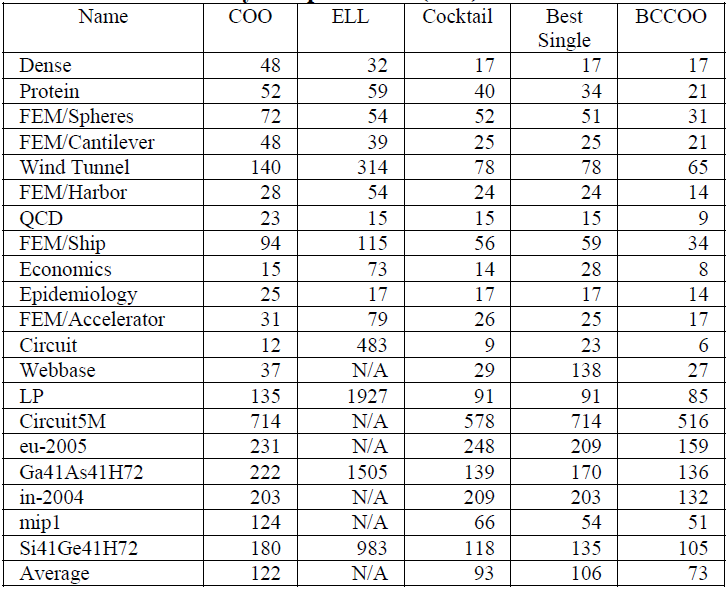
\includegraphics[scale=0.4]{figure/fig6-memoryprint.png}
	\end{figure}
\end{frame}

\subsection{Performance Comparison}
\begin{frame}
	\frametitle{Performance Comparison between Other Algorithms}
	\begin{figure}
		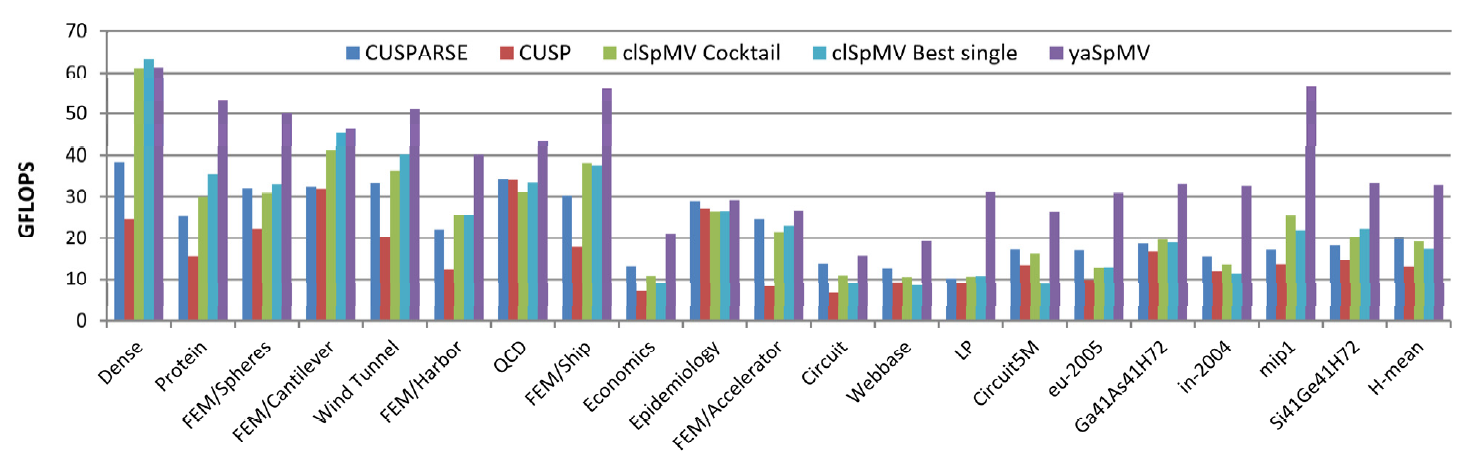
\includegraphics[scale=0.25]{figure/fig7-exp1.png}
	\end{figure}
\end{frame}

\begin{frame}
	\frametitle{Performance Comparison between Different Optimizations}
	\begin{figure}
		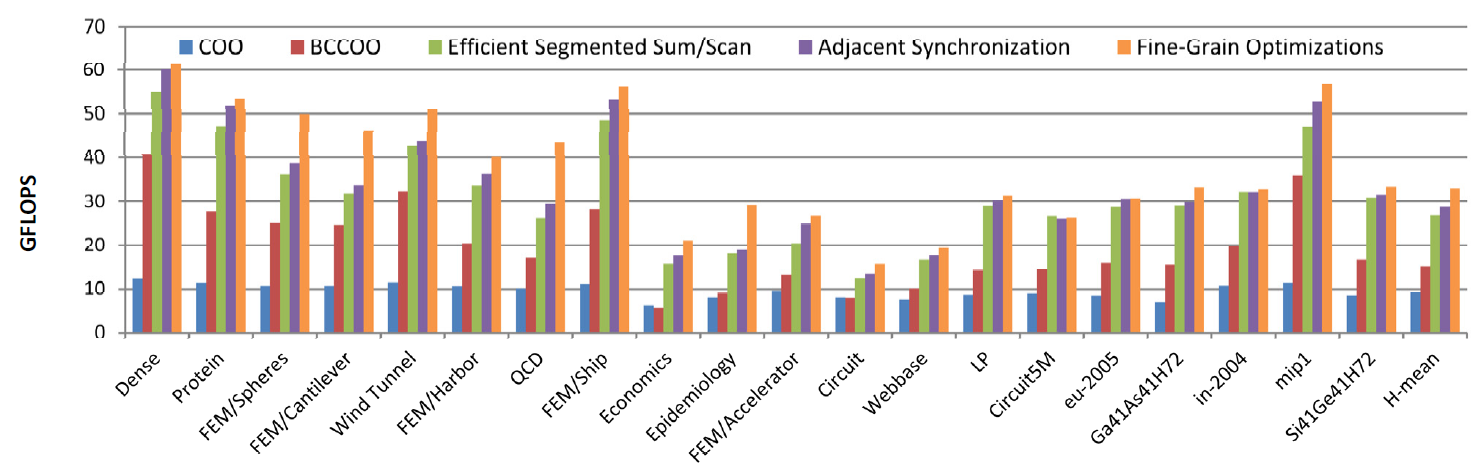
\includegraphics[scale=0.25]{figure/fig8-exp2.png}
	\end{figure}
\end{frame}
\section{Extension to Distributed Memory}

\subsection{SDSM Framework Introduction}
\begin{frame}
    \frametitle{SDSM Framework}
    	Novel shared-distributed-shared-memory (SDSM) 
    	framework uses
    \begin{itemize}
    	\item Hierarchical dynamic load-balancing,
    	\item Work-stealing
    \end{itemize}
     	to balance the load among the processes for our CORDAC algorithms.
\end{frame}

\subsection{SDSM: Multi-level Hierarchy}
\begin{frame}
    \frametitle{Multi-level Hierarchy}
    If we have $K$ processes,
    \begin{itemize}
    	\item a super-master,
    	\item some $M'$ of them as masters, and
    	\item the rest as workers.
    \end{itemize}
    They run multithreaded code on $p$ cores.
\end{frame}

\begin{frame}
    \frametitle{Shared Job Queue}
    \begin{itemize}
    	\item Each super-master/master process maintains a shared 
    		job queue.
    	\item If a thread run a function on input size
            \footnote{$\textit{min offload threshold} \le x \le \textit{max offload threshold}$}
             $x$, 
    		try to lock the job queue and put at most $l-1$
    		out of its $l$ parallellly executable recursive sub-divisions in job queue.
    	\item If a thread waits its submitted jobs finished,
    		it steals back its latest submitted jobs left in the job queue.
    \end{itemize}
\end{frame}

\subsection{SDSM: Result}
\begin{frame}
    \frametitle{Result}
    \begin{figure}
		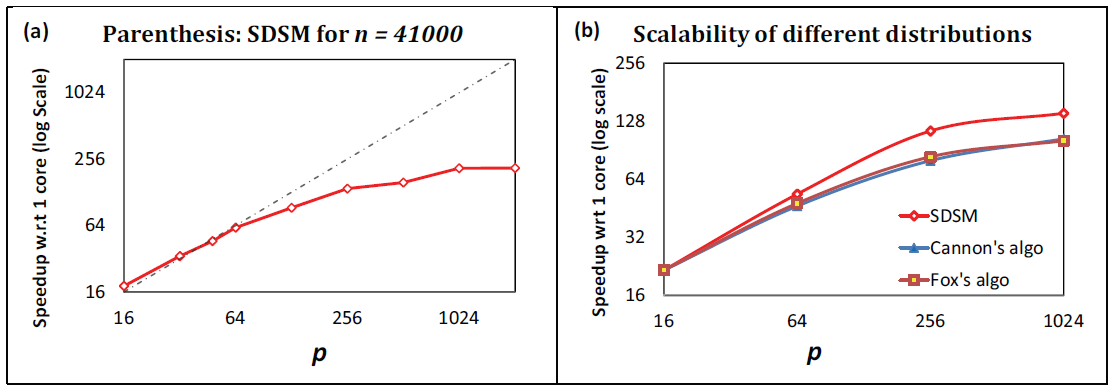
\includegraphics[scale=0.3]{figure/fig-distributed-result.png}
	\end{figure}
    \begin{itemize}
    	\item For parenthesization problem, we fixed $n = 41 K$ and 
    		allowed offloading of problems with a size in the range of
    		$256$ -- $2048$.
    \end{itemize}
\end{frame}

\end{document}
